\documentclass{lzureport}
%\usepackage{enumerate}

\major{计算数学}
\name{甄继伟}
\title{期末复习}
\stuid{2001312001}
\college{麻省理工大学}
\date{\zhtoday}
\expname{期末复习}
\course{深度学习}


\begin{document}

\makecover

%\input{chapter/abstract.tex}

\thispagestyle{empty}
\tableofcontents
\newpage 
\setcounter{page}{1}
\setcounter{equation}{0} % 重置公式计数器

%%%%%%%%%%%%正文
\section{卷积定理}
\begin{Thm}[卷积定理]
	已知两个时域(频域)信号
	$$
	\begin{aligned}
		&\mathscr{F}[f_{1}(t)] =F_{1}(f)  \\
		&\mathscr{F}[f_{2}(t)] =F_2(f)  
	\end{aligned}
	$$
	那么
	$$
	\mathscr{F}\left[f_1(t)*f_2(t)\right]=F_1(f)\cdot F_2(f)
	$$
\end{Thm}	
卷积定理指出,

\colorbox{yellow}{\color{black}\textcolor{YBXPurple}{函数卷积的傅里叶变换}是\textcolor{YBXPurple}{函数傅立叶变换的乘积}}。

具体分为时域卷积定理和频域卷积定理,

\textcolor{YBXPurple}{时域卷积定理}即\textcolor{YBXPurple}{时域}内的卷积对应频域内的乘积;

\textcolor{YBXPurple}{频域卷积定理}即\textcolor{YBXPurple}{频域}内的卷积对应时域内的乘积,两者具有对偶关系。

傅里叶变换公式:\colorbox{yellow}{\color{black}$\mathscr{F}[f(t)]=F(f)=\int_{-\infty}^{\infty}f(t)e^{-j2\pi ft}dt$}

\begin{derivation}{证明时域卷积定理}
	$
	\begin{aligned}
		\mathscr{F}[f_{1}(t)*f_{2}(t)]&=\int_{-\infty}^{\infty}f_{1}(t)*f_{2}(t)e^{-j2\pi ft}dt \\
		&=\int_{-\infty}^{\infty}\int_{-\infty}^{\infty}f_{1}(\tau)f_{2}(t-\tau)d\tau e^{-j2\pi ft}dt \\
		&=\int_{-\infty}^{\infty}\int_{-\infty}^{\infty}f_2(t-\tau)e^{-j2\pi ft}dtf_1(\tau)d\tau  \\
		&\overset{x=t-\tau}{=}\int_{-\infty}^{\infty}\int_{-\infty}^{\infty}f_2(x)e^{-j2\pi f(x+\tau)}dxf_1(\tau)d\tau \\
		&=\int_{-\infty}^{\infty}\int_{-\infty}^{\infty}f_2(x)e^{-j2\pi f\tau}e^{-j2\pi fx}dxf_1(\tau)d\tau  \\
		&=\int_{-\infty}^\infty f_2(x)e^{-j2\pi fx}dx\int_{-\infty}^\infty f_1(\tau)e^{-j2\pi f\tau}d\tau  \\
		&=F_1(f)\cdot F_2(f)
	\end{aligned}$
\end{derivation}

\subsection{卷积的保范性和保角性}
\subsubsection{保范性(Isometry)}
卷积操作和信号能量的关系

考虑离散信号$x[n]$和卷积核$h[n]$的卷积定义为:
$$(x*h)[n]=\sum_kx[k]h[n-k]$$

信号的范数(能量)通常用二范数表示:
$$\|x\|_2=\left(\sum_n|x[n]|^2\right)^{1/2}$$

卷积后信号的能量可以表示为:
$$\|y\|_2=\|x*h\|_2$$
根据帕塞瓦尔定理 (Parseval's Theorem),卷积后信号的能量与输入信号和卷积核的能量

有关:
$$\|x*h\|_2^2=\|x\|_2^2\cdot\|h\|_2^2$$
这意味着卷积操作后信号的能量是输入信号和卷积核能量的乘积,而不会引入过大的能量变化,从而体现了卷积的保范性。

\subsubsection{保角性(Conformality)}
卷积的保角性主要体现在它的平移不变性和局部一致性上。

\begin{enumerate}[label=\arabic*)]
	\item 平移不变性:\\

	考虑一个信号$x[n]$和它的平移$x[n-n_0]$,以及卷积核$h[n]$。它们的卷积可以表示为:
	$$\begin{aligned}&(x*h)[n]=\sum_kx[k]h[n-k]\\&(x[n-n_0]*h)[n]=\sum_kx[k-n_0]h[n-k]\end{aligned}$$
	
	通过变量替换$k^{\prime}=k-n_0$,我们有:
	$$(x[n-n_0]*h)[n]=\sum_{k^{\prime}}x[k^{\prime}]h[n-k^{\prime}-n_0]=(x*h)[n-n_0]$$
	
	这说明卷积操作具有平移不变性,即卷积后的结果仅是平移的输入信号的平移。

	\item 局部一致性:\\
	卷积操作在局部区域内进行计算,即每个输出值仅依赖于卷积核覆盖的输入信号的局部区域。对于小的输入变化(如噪声或局部扰动),卷积后的输出不会发生剧烈变化。这种局部一致性可以通过观察卷积和相关运算 (如边缘检测)的输出变化情况来验证。
\end{enumerate}

\subsection{卷积加速}
\subsubsection{快速傅里叶变换(FFT)}
快速傅里叶变换(FFT)是一种高效的计算傅里叶变换的方法,它可以将离散信号的傅里叶变换计算复杂度从$O(N^2)$降低到$O(N\log N)$。

对于长度为$N$的离散信号$x[n]$,其傅里叶变换可以表示为:
$$X[k]=\sum_{n=0}^{N-1}x[n]e^{-j2\pi kn/N}$$

FFT算法的基本思想是将信号分解为奇数点和偶数点的和,然后递归地计算每个子序列的傅里叶变换。

卷积定理的FFT加速

卷积定理可以通过FFT加速卷积运算,具体步骤如下:
\begin{enumerate}[label=\arabic*)]
	\item 对输入信号$x[n]$和卷积核$h[n]$进行零填充,使其长度为$2N$。
	\item 分别计算$x[n]$和$h[n]$的FFT,得到$X[k]$和$H[k]$。
	\item 计算卷积结果$Y[k]=X[k]\cdot H[k]$。
	\item 对$Y[k]$进行逆FFT,得到卷积结果$y[n]$。
\end{enumerate}

\subsubsection{卷积加速应用}
\begin{enumerate}[label=\arabic*)]
	\item 参数共享:\\
	卷积层中的卷积核(滤波器)在整个输入图像上滑动应用同一组参数(权重)。
	
	这意味着卷积层中的参数数量大大减少,避免了全连接层中每个输入像素和每个输出像素之间都需要单独参数的问题,从而减少了计算和存储需求。
	\item 稀疏连接:\\
	卷积操作只考虑局部感受野内的像素,这意味着每个输出单元只与输入图像中的一小部分像素连接,而不是与所有像素连接。
	
	这种稀疏连接不仅减少了计算量,还保留了图像的局部特征。
	\item 高效的前向传播和反向传播:\\
	卷积操作可以通过高效的矩阵运算库(如BLAS、cuDNN等)进行实现,利用GPU的并行计算能力,大大加速了前向传播和反向传播的计算过程。
\end{enumerate}



\newpage
\section{人脸检测网络}
目标检测两大流派诞生了:一个是以R-CNN为始祖的two-stage派系,一个是以YOLO为始祖的one-stage派系。
前者往往准确度更高但速度上较慢,后者往往更快但准头略差一些。

\subsection{两步法}

\begin{figure}[htpb]
	\centering
	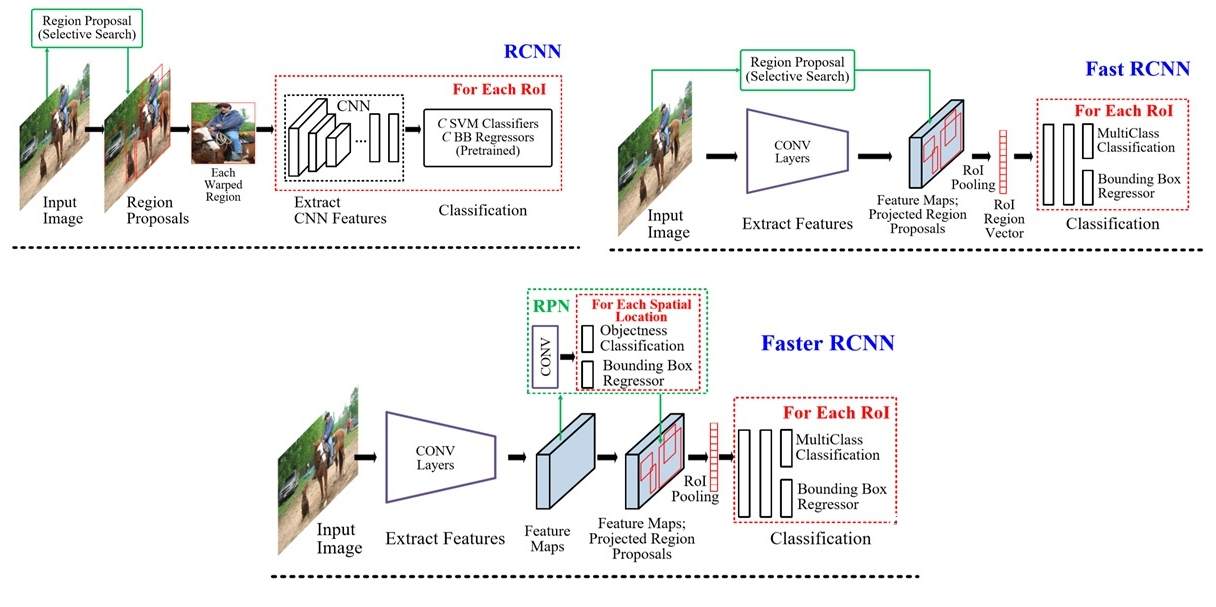
\includegraphics[width=0.6\textwidth]{figure/RCNN图谱.png}
	\caption{RCNN图谱}
	\label{fig:RCNN图谱}
\end{figure}


两步法(Two-Stage Method)是一种逐步细化和筛选的方法,主要包括两个阶段:

\begin{enumerate}[itemindent=1em,label=\arabic*)]
	\item 候选区域生成\\
	从输入图像中提取人工视觉特征(如HOG)

	比如通过 \textcolor{YBXPurple}{积分图像}找到眼睛的候选区域
	\item 特征提取\\
	将提取出的视觉特征输入给分类器(如SVM)进行分类。
\end{enumerate}


\subsection{YOLO}
YOLO(You Only Look Once)方法是一种单步法(Single-Stage Method),它将检测和分类任务结合在一个神经网络中。

YOLO的基本思想是将整个图像分成多个网格,每个网格直接预测包含对象的边界框和类别。

YOLO并没有真正去掉候选区域,而是创造性的将候选区和目标分类合二为一

最大的特点就在于:仅使用一个卷积神经网络端到端地实现检测物体的目的。其网络整体的结构如图\ref{fig:YOLOv1网络结构}所示。
\begin{figure}[htpb]
	\centering
	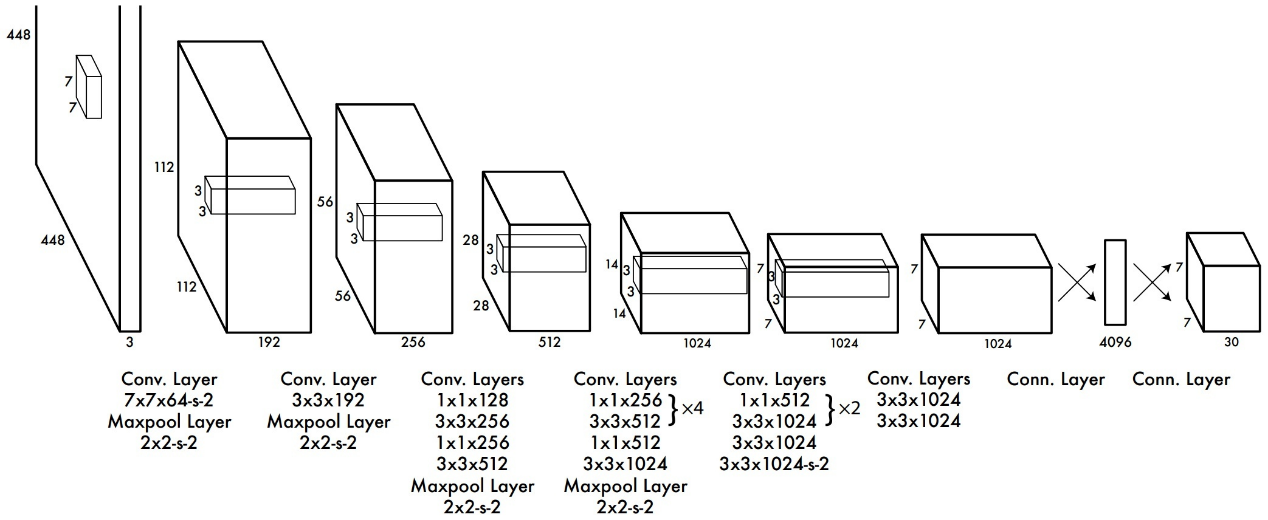
\includegraphics[width=0.6\textwidth]{figure/YOLOv1网络结构.png}
	\caption{YOLO v1网络结构}
	\label{fig:YOLOv1网络结构}
\end{figure}






\newpage
\section{降噪复原网络}
\subsection{传统方法}
我们考虑如下形式的图像复原问题:
$$y=f*h+\eta $$
其中:
 \begin{enumerate}[itemindent=1em,label=\arabic*)]
	\item $y$表示观测到的模糊图像。
	\item $f$表示原始的未模糊图像。
	\item $h$表示点扩散函数(Point Spread Function,PSF),描述了图像的模糊过程
	\item $\eta$表示加性噪声。
 \end{enumerate}
 
 通过快速傅里叶变换(FFT),上述卷积操作可以转化到频域表示:
 $$\bar{y}=\hat{f}\cdot\hat{h}+\hat{\eta}$$
 
 其中:
$\bar{y} , \hat{f} , \hat{h}$和$\hat{\eta}$分别是$y,f,h$和$\eta$的频域表示。

将观测图像$\hat{y}$除以点扩散函数$\hat{h}$,可以得到原始图像的估计加上一个噪声项的比值。

$$\frac{\hat{y}}{\hat{h}}=\hat{f}+\frac{\hat{\eta}}{\hat{h}}$$

维纳滤波器公式的推导
$$\frac{\hat{y}\cdot\hat{h}^*}{\hat{h}\cdot\hat{h}^*}$$
其中$\hat{h}^*$表示$\hat{h}$的共轭复数。这个操作是为了处理频域中的卷积,并且它有助于消除频谱中的噪声。

维纳滤波器公式
$$\frac{\hat y\cdot\hat h^*}{|\hat h|^2+\lambda}\approx\hat f+\frac{\hat\eta}{\hat h}$$

这个公式引入了一个正则化参数$\lambda$,其目的是平衡信号与噪声的贡献。具体而言,维纳滤波器通过如下公式来实现图像复原:

$$\hat{f}=\frac{\hat{y}\cdot\hat{h}^*}{|\hat{h}|^2+\lambda}$$

\begin{enumerate}[label=\arabic*)]
	\item $\frac {\hat{y} \cdot \hat{h} ^* }{| \hat{h} | ^2+ \lambda }:$

	分子$\hat{y}\cdot\hat{h}^*$是观测图像与点扩散函数的共轭复数相乘。
	
	分母$|\hat{h}|^2+\lambda$是点扩散函数的频谱强度加上正则化参数。
	\item 正则化参数$\lambda $

	$\lambda$控制了噪声抑制的程度。如果$\lambda$过小,可能会放大噪声;如果$\lambda$过大,可能会导致图像模糊。
	
	选择合适的$\lambda$能在图像复原和噪声抑制之间取得平衡。
	\item 结果近似为:
	
	$\hat{f}+\hat{\eta}$,这表示复原后的图像包含了原始图像的频域表示加上噪声的影响。
\end{enumerate}


\subsection{使用CNN原理}
使用卷积神经网络(CNN)进行图像降噪和复原是一种有效的方法。CNN能够通过学习提取图像的各种特征,进而对噪声进行滤除,并恢复原始图像。

CNN网络通常包括卷积层、池化层、激活函数、全连接层等组件,通过这些组件的组合,CNN网络能够学习到图像的特征,从而实现图像降噪和复原。


\subsubsection{CNN网络结构设计}
设计一个用于图像降噪的卷积神经网络,主要包括以下几个部分:
\begin{enumerate}[label=\arabic*)]
	\item 输入层:

	接收含噪声的图像,通常是一个灰度图像(单通道)或彩色图像(三通道)。

	\item 编码器部分:
	\begin{enumerate}[itemindent=1em,label=(\arabic*)]
		\item 多个卷积层:\\
		选择合适的卷积核大小(通常为3x3或5x5),以平衡特征提取的细节和计算效率。

		使用多个卷积层提取图像特征,每个卷积层后接ReLU激活函数以增加非线性。

		\item 批量归一化层:\\
		在卷积层之后加入批归一化层,对卷积层的输出进行归一化,以稳定和加速训练过程。

		\item 使用最大池化层进行下采样:\\
		使用池化层(如最大池化)进行下采样,以降低特征图的分辨率并增加感受野
	\end{enumerate}

	\item 中间处理部分:
	\begin{enumerate}[itemindent=1em,label=(\arabic*)]
		\item 多个卷积层:\\
		在编码器部分之后,再次使用多个卷积层提取更高级的特征。

		\item 批量归一化层:\\
		每个卷积层后接ReLU激活函数和批归一化层。
	\end{enumerate}

	\item 解码器部分:
	\begin{enumerate}[itemindent=1em,label=(\arabic*)]
		\item 上采样:\\
		使用转置卷积层(Transpose Convolution)进行上采样,将特征图的分辨率恢复到原始大小。

		\item 批量归一化层:\\
		每个转置卷积层后接ReLU激活函数和批归一化层。

		\item 特征图映射回像素空间:\\
		使用卷积层将特征图映射回原始图像的像素空间,以恢复去噪后的图像。
	\end{enumerate}
	
	\item 输出层:
	输出去噪后的图像。
\end{enumerate}

\newpage
\section{棋盘格角点检测网络}
\textcolor{blue}{\textbf{角点检测}}: 主要目的是在图像中找到特征明显的角点位置。这些角点通常是图像中具有高梯度变化的点,如图像中的边缘、角落等。角点检测提供的是像素级别的精度。

\textcolor{blue}{\textbf{亚像素估计}}: 主要目的是在已经检测到的角点的基础上,进一步提高这些点的位置精度。亚像素估计使得角点位置的精度超越像素级别,达到亚像素级别。

\subsection{构造棋盘格}
先通过随机数找到棋盘格的角点,然后通过这些角点构造棋盘格。

\subsubsection{方法一}
如果生成小数点后两位的坐标,可以通过以下代码生成棋盘格:
\begin{enumerate}[itemindent=1em,label=\arabic*)]
	\item 先扩大成100倍,然后取整
	\item 生成棋盘格
	\item 缩小100倍
\end{enumerate}

\subsubsection{方法二}
如果生成小数点后两位的坐标,
\begin{figure}[htpb]
	\centering
	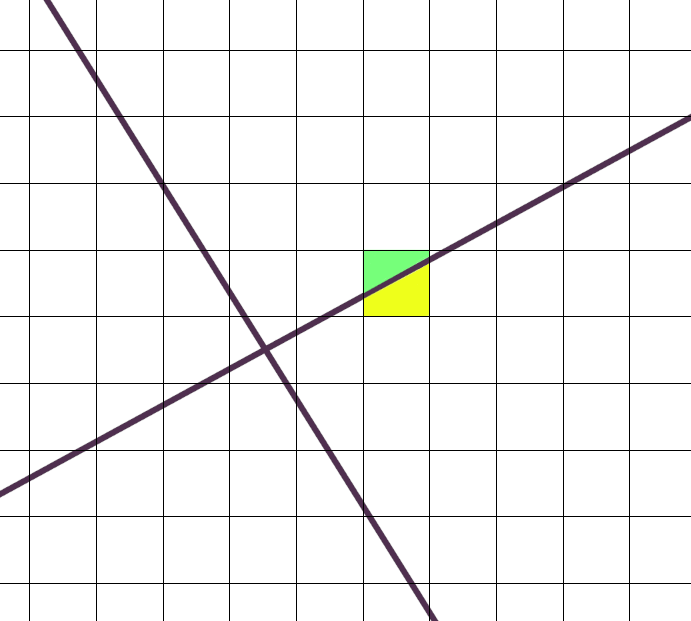
\includegraphics[width=0.6\textwidth]{figure/生成角点图.png}
	\caption{生成角点图}
	\label{fig:生成角点图}
\end{figure}

\begin{enumerate}[label=\arabic*)]
	\item 如图\ref{fig:生成角点图}所示,先通过角点做出两条互相垂直的直线\\
	这里输入层是一个32x32的矩阵,每个像素点的值是0-1之间的浮点数	
	\item 这两条直线在像素坐标相交的位置,需要对像素进行赋值\\
	以图中直线为例,该像素的赋值取决于黄色区域与绿色区域的面积比
	\item 记录角点在像素内的偏移量($x_1, x_2$)
	\item 对像素区域施加 Gauss模糊,记录在32x32矩阵	
\end{enumerate}

\subsection{角点检测}
角点(corner)是图像中局部区域具有显著变化的点,通常位于边缘的交叉点或纹理丰富的区域。

\subsubsection{张忠波老师的土方法}
将矩阵进行旋转$180^{\circ}$,然后与原矩阵按位相减,计算误差,误差越小的点越有可能是角点。

\subsubsection{Harris角点检测}
Harris角点检测(Harris Corner Detection)是一种基于局部区域的角点检测方法,
它通过计算局部区域的灰度变化来检测角点。

Harris角点检测的\textcolor{YBXPurple}{基本思想}是通过计算图像灰度变化的矩阵特征值来识别角点。

\begin{enumerate}[label=\arabic*)]
	\item 梯度计算:计算图像在水平和垂直方向上的梯度。通常使用Sobel算子进行滤波,得到梯度图像$I_x$和$I_y$。

	Sobel算子进行滤波的过程如下:
	\begin{enumerate}[itemindent=1em,label=(\arabic*)]
		\item Sobel算子在水平方向和垂直方向上分别使用两个3x3的卷积核,这两个卷积核用于计算图像在这两个方向上的梯度。

		水平方向(x方向)的Sobel算子:
		$$G_x=\begin{bmatrix}-1&0&1\\-2&0&2\\-1&0&1\end{bmatrix}$$
		
		垂直方向(y方向)的Sobel算子:
		$$G_y=\begin{bmatrix}-1&-2&-1\\0&0&0\\1&2&1\end{bmatrix}$$
		\item 灰度化图像:如果输入图像是彩色图像,首先将其转换为灰度图像。这一步通过加权平均RGB通道来完成:
		$$M_{\mathrm{gray}}=0.299\cdot R+0.587\cdot G+0.114\cdot B$$

		\item 卷积运算:分别使用水平和垂直方向的Sobel算子对灰度图像进行卷积运算,得到水平方向和垂直方向的梯度图像$I_x$和$I_y$。
		$$
		\begin{aligned}I_x(x,y)&=\sum_{i=-1}^1\sum_{j=-1}^1G_x(i+1,j+1)\cdot M(x+i,y+j)\\
			I_y(x,y)&=\sum_{i=-1}^1\sum_{j=-1}^1G_y(i+1,j+1)\cdot M(x+i,y+j)
		\end{aligned}
		$$
		这里 $M(x,y)$ 表示灰度图像的像素值。$I_x$ 和 $I_y$ 分别表示图像在水平和垂直方向上的梯度。 $G_x(i+1, j+1)$ 和 $G_y(i+1, j+1)$ 分别表示Sobel算子的卷积核中的元素。

		\item 梯度幅度和方向:计算梯度图像的幅度和方向。
		计算每个像素点的梯度幅值和梯度方向。梯度幅值可以表示边缘的强度,梯度方向表示边缘的方向。

		梯度幅值:
		$$G=\sqrt{G_x^2+G_y^2}$$

		梯度方向:
		$$\theta=\arctan\left(\frac{G_y}{G_x}\right)$$
	\end{enumerate}
	
	\item 构建结构张量(第二矩阵):计算结构张量 $M$,其中包含局部窗口内的梯度信息。
	$$M=\begin{bmatrix}\sum I_x^2&\sum I_xI_y\\\sum I_xI_y&\sum I_y^2\end{bmatrix}$$

	\item 计算角点响应函数:通过计算结构张量的特征值来判断是否为角点。

	通过结构张量的特征值计算角点响应函数$R:$
	$$R=\det(M)-k\cdot(\mathrm{trace}(M))^2$$
	其中,$\det(M)=\lambda_1\lambda_2$是矩阵$M$的行列式,$\operatorname{trace}(M)=\lambda_1+\lambda_2$是矩阵$M$的迹,$\lambda_1$和$\lambda_2$是结构张量的特征值,$k$是一个经验参数,通常取值在 0.04 到 0.06 之间。

	\item 非极大值抑制:对角点响应函数进行非极大值抑制,保留局部最大值点作为角点。
	
	具体做法
	\begin{enumerate}[itemindent=1em,label=(\arabic*)]
		\item 对每个像素计算角点响应函数值。
		\item 对响应值进行阈值处理,去除小于阈值的响应。
		\item 在局部区域内保留响应值最大的像素点,其他点置零。
	\end{enumerate}
	
\end{enumerate}

\subsubsection{CNN方式}
CNN网络结构设计

输入图像 -> 卷积层(Conv1) + ReLU -> 最大池化层(Max Pool1) -> 卷积层(Conv2) + ReLU -> 最大池化层(Max Pool2) -> 全连接层(FC1) -> 输出层(Output)

\begin{enumerate}[label=\arabic*)]
	\item 输入层:
	\begin{enumerate}[itemindent=1em,label=(\arabic*)]
		\item 输入数据:尺寸为32x32的灰度图像。
		\item 功能:提供图像数据给后续的卷积层进行特征提取。
	\end{enumerate}
	\item 第一卷积层(Conv1):
	\begin{enumerate}[itemindent=1em,label=(\arabic*)]
		\item 卷积核大小:5x5\\
		选择5x5的卷积核大小是因为其能够捕捉较大的局部特征,适合提取图像中的重要信息。
		\item 输出通道数:6\\
		采用多个卷积核(6个)是为了提取多种不同的特征,从而增加模型的鲁棒性。
		\item 步长(stride):1
		\item 填充(padding):1
		\item 激活函数:ReLU\\
		使用ReLU激活函数是因为其计算简单且能有效解决梯度消失问题,促进深层网络的训练。
		\item 功能与目的:卷积层的主要目的是通过局部感知获取图像的局部特征,提取低级特征如边缘、角点等。通过使用多个卷积核,可以提取不同类型的特征。ReLU激活函数引入非线性,增加模型的表达能力。
	\end{enumerate}
	\item 第一最大池化层(Max Pool1):
	\begin{enumerate}[itemindent=1em,label=(\arabic*)]
		\item 池化核大小:2x2\\
		采用2x2的最大池化层是因为其可以显著减少特征图的尺寸,同时保留重要的特征信息,避免过拟合。
		\item 步长(stride):2
		\item 功能与目的:最大池化层通过对特征图进行下采样,减小特征图的尺寸,提高模型的计算效率。同时,最大池化层还能增加模型的平移不变性,提高模型的泛化能力。
	\end{enumerate}
	\item 第二卷积层(Conv2):
	\begin{enumerate}[itemindent=1em,label=(\arabic*)]
		\item 卷积核大小:5x5
		\item 输出通道数:6
		\item 步长(stride):1
		\item 填充(padding):0
		\item 激活函数:ReLU
		\item 功能与目的:第二卷积层继续提取图像的高级特征,如纹理、形状等。通过增加输出通道数,可以提高模型的表达能力。ReLU激活函数引入非线性,增加模型的表达能力。
	\end{enumerate}
	\item 第二最大池化层(Max Pool2):
	\begin{enumerate}[itemindent=1em,label=(\arabic*)]
		\item 池化核大小:2x2
		\item 步长(stride):2
		\item 功能与目的:第二最大池化层通过对特征图进行下采样,减小特征图的尺寸,提高模型的计算效率。同时,最大池化层还能增加模型的平移不变性,提高模型的泛化能力。
	\end{enumerate}
	\item 全连接层(FC1):
	\begin{enumerate}[itemindent=1em,label=(\arabic*)]
		\item 输出节点数:20
		\item 功能与目的:将卷积层和池化层提取到的特征映射到一个更高维度的空间,以便于进行最终的回归任务。全连接层通过学习特征之间的全局关系,提高模型的判别能力。	\\
		通过全连接层将卷积和池化层提取的特征映射到更高维度的空间,从而实现对角点坐标的精确预测。
	\end{enumerate}
	\item 输出层(Output):
	\begin{enumerate}[itemindent=1em,label=(\arabic*)]
		\item 输出节点数:2(对应角点的坐标(u, v))
		\item 功能与目的:输出层通常用于回归任务,输出模型的预测结果。在角点检测任务中,输出层输出角点的坐标。
	\end{enumerate}		
	
	\item 计算损失函数
	$$Loss = \frac{1}{2}[(x_1 - u)^2 + (x_2 - v)^2]$$

	利用梯度下降法更新权重,使得损失函数最小化。

	重复训练过程,直到模型收敛,得到最优的权重参数。

	
\end{enumerate}

\newpage
\section{图像盲复原}
\subsection{盲复原问题}
图像盲复原是指在点扩散函数(PSF)未知的情况下,对退化图像进行复原的过程。盲复原的挑战在于同时估计出模糊核和清晰图像,而非盲复原则只需在已知模糊核的情况下恢复图像。盲复原在许多实际应用中具有重要意义,如天文图像处理、医疗成像和遥感图像分析。

\subsection{模糊核估计}
模糊核(PSF)是导致图像模糊的关键因素。盲复原的首要任务是估计模糊核的形状和参数。

\begin{enumerate}[label=\arabic*)]
	\item 离焦模糊:模糊核为均匀圆盘。离焦模糊通常由成像系统的焦距误差引起。
	\item 高斯模糊:模糊核为高斯分布,常见于大气湍流和光学系统的点扩散。
	\item 运动模糊:模糊核为直线,通常由成像过程中相机的线性运动引起。复杂的运动模糊涉及更复杂的模糊核形状。
\end{enumerate}

\subsection{估计方法}
\begin{enumerate}[label=\arabic*)]
	\item 直接法:适用于特殊点扩散函数类型,通过已知的物理特性和先验知识直接估计模糊核的参数。
	\item 循环迭代法:常用于一般盲复原问题。首先假设一个模糊核,复原图像,然后利用复原图像更新模糊核。反复迭代直到收敛。
\end{enumerate}

\subsection{正则化复原}
正则化技术用于约束复原问题,使其更具稳定性和解的唯一性。

全变差正则化:通过最小化图像梯度的全变差,保持图像的边缘信息。

数学模型:$\min_{k,L}\left(\|B-k*L\|^2+\alpha\|\nabla L\|+\beta\|\nabla k\|\right)$

分离变量法:将全变差问题分解为两个子问题,通过交替最小化求解。

\subsection{多尺度方法}
多尺度方法通过在不同尺度上估计模糊核,从而提高估计的精度和稳定性。

步骤
\begin{enumerate}[label=\arabic*)]
	\item 从粗略尺度开始估计模糊核和图像。
	\item 逐步细化尺度,利用前一尺度的结果作为下一尺度的初始值。
	\item 在最细尺度上完成最终的模糊核和图像估计。
\end{enumerate}

\newpage
\section{畸变矫正函数}
畸变矫正是一个重要的研究方向。畸变是指由于摄像头镜头的非理想特性导致图像中的几何失真。

1.方程与初始条件:
$$\begin{aligned}
	\left\{\begin{matrix}
	&r=\sqrt{u^2+v^2}\\
	&U_d=u+(u+k_1r^2+k_2r^4+k_3r^6)+P_1(u^2+r^2)+S_xr^2\\
	&V_d=v+(v+k_1r^2+k_2r^4+k_3r^6)+P_2(v^2+r^2)+S_yr^2
	\end{matrix}\right.
	\end{aligned}$$
	这里,$k_1,k_2,k_3,P_1,P_2,S_x,S_y$为待优化参数($k_1,k_2,k_3$为径向畸变系数;$P_1,P_2$为切向畸变系数;$S_x,S_y$为缩放参数),$U_d,V_d$ 为目标矫正点,$r$表示点$(u,v)$到图像中心的距离。


2. 目标函数:
	$$J(u,v)=\int f(u,v-U_d)-g(u,v-V_d)$$

	$J(u,v)$表示校正后的误差,$f,g$为误差函数。

3. 数值解法:

$$J_{u,v}=f(u,v-U_d)+g(u,v-V_d)^2$$

我们通过计算每个像素点的误差来调整参数。

4.梯度下降法:
$$\Delta w_j^{(t+1)}=-\eta\frac{\partial E}{\partial w_j^{(t)}}$$	

其中,当 $\frac{\partial E}{\partial w_j^{(t)}} > 0$ 时,$\Delta w_j^{(t)}$ 增大,
当 $\frac{\partial E}{\partial w_j^{(t)}} < 0$ 时,$\Delta w_j^{(t)}$ 减小。

\subsection{算法流程}
\begin{enumerate}[label=\arabic*)]
	\item 令 $(u, v)$ 代入值,得到输出 $(U_d, V_d)$。
	\item 用 $(U_d, V_d)$ 作为初始值。
	\item 构建输入与输出之间的关系,逐步逼近最优解。
	\item 更新公式:
	$$
	\begin{aligned}
		&U_{ij}& =u_{ij}+u_{ij}k_1r_{ij}^2+k_2r_{ij}^4+k_3r_{ij}^6+P_1u_{ij}^2+S_xr_{ij}^2  \\
		&V_{ij}& =v_{ij}+v_{ij}k_1r_{ij}^2+k_2r_{ij}^4+k_3r_{ij}^6+P_2v_{ij}^2+S_yr_{ij}^2  \\
	\end{aligned}
	$$
	\item 误差计算:
	$$\mathrm{Loss}=\sum(U_{ij}-CU_{ij})^2+(V_{ij}-CV_{ij})^2$$

	\item 收敛条件:
	Loss 收敛时(小于预设的阈值),停止迭代。
\end{enumerate}




\end{document}